\documentclass[12pt]{article}

\usepackage{epsf}
\usepackage{color}
\usepackage{amsmath}
\usepackage{graphicx}
\usepackage[colorlinks,urlcolor=blue,citecolor=blue,linkcolor=blue]{hyperref}
\usepackage{natbib}
\usepackage{sidecap}

\usepackage{outlines}
\usepackage{enumitem}
\setenumerate[1]{label=\Roman*.}
\setenumerate[2]{label=\Alph*.}
\setenumerate[3]{label=\roman*.}
\setenumerate[4]{label=\alph*.}


\setlength{\oddsidemargin}{0.25in}
\setlength{\textwidth}{6.5in}
\setlength{\topmargin}{0in}
\setlength{\textheight}{8.5in}

\bibliographystyle{apj}
\citestyle{aa}

\input{commands.tex}

%Commands specific to the this work
\newcommand{\editorial}[1]{\textcolor{red}{#1}}

\begin{document}

\title{Galaxy Cluster Dynamics in the Era of Large Spectroscopic Surveys}
\author{Steven Boada}
\date{\today}

\maketitle

\section{Introduction}\label{sec:introduction}
Clusters of galaxies form the largest bound objects in the universe, and as such their study is a cornerstone in modern day astronomy. First recognized by 19th century astronomers, their place in astronomical canon was solidified when Edwin Hubble proofed their constituent nebulae where not bound to the Milky Way \citep{Hubble1926} but collections of stars similar to the Milky Way. Work to understand their nature and origin began in ernest when \cite{Hubble1931} used the virial theorem and the galaxy velocities in the centers of the Virgo \citep{Smith1936} and Coma \citep{Zwicky1933} clusters to derive their masses. The immense mass derived exceeded the total stellar mass contributed by all galaxies many times over. This lead Zwicky to theorize the existence of large amounts of non-luminous matter, and coining the term ``dark matter'' (DM), which we still use today.  

Modern astronomy gives the composition of galaxy clusters in three many parts. The galaxies themselves comprise the most obvious feature, and contain a large portion (but not the entirety) of the luminous matter (stars) in the cluster. The intracluster medium (ICM) is the space between the cluster galaxies and is composed many of ordinary matter (baryons) which are super heated to tens of thousands of kelvin. The ICM contains the bulk of the cluster's baryonic matter, and while it is very hot, it is not very dense, with a typical value of $10^{-3}$ particles per cubic centimeter. The majority of the cluster's mass is located in the DM halo which surrounds the cluster. 

Thought to form out of the primordial density fluctuations in the very early universe, the investigation of their formation and growth began in the 1960s. Soon thereafter, the hierarchical model of structure formation \citep{Press1974, Gott1975, White1978} was introduced. It suggests the first stars and stellar clumps grew first then subsequently merged together with dark matter and other gas clumps to form the first galaxies which then continued to merge and grow into the clusters and large scale structures we see today. This accretion of smaller systems is thought to be driven by the gravity of the DM associated with the cluster. Of course, many complicated astrophysical processes are at work during cluster growth and similarly complicated theoretical models seek to explain these processes. For a detailed review of cluster formation see \cite{Kravtsov2012}.

The number and distribution of galaxy clusters across the sky is the finger print of the cosmology imprinted on the universe at its birth. To uncover the underlying cosmology a detailed understanding of the astrophysical processes that describe the motion of constituent galaxies and their impact on the ICM is required. So, galaxy clusters stand at the intersection of cosmology and astrophysics. 

\subsection{Cluster Cosmology}
The current concordance cosmology is a parametrization of the Big Bang cosmological model where the universe contains a cosmological constant ($\Lambda$; often referred to as dark energy) and cold dark matter (CDM). It is often characterized by six parameters; the Hubble Constant ($H_0$), the baryonic matter density ($\Omega_b$), the dark matter density ($\Omega_c$), the dark energy density ($\Omega_\Lambda$); the normalization of the power spectrum ($\sigma_8$); the spectral index of the power spectrum ($n_s$). Galaxy clusters are sensitive probes of $\Omega_m$, the total mass ($\Omega_b + \Omega_c$) density in the universe, through tracing the peaks in the universal matter density often referred to as the power spectrum of matter density fluctuations or the matter power spectrum and $\sigma_8$ by the comparison of the number density of observed halos to that predicted in cosmological models. %Although, in reality, one measures $\sigma_8\Omega_m^\alpha$, where the value of $\alpha$ depends on the masses of the halos considered.

The determination of cosmological parameters is done by comparing the number of galaxy clusters per unit mass per unit comoving volume ($n(M,z)$) to models. See \cite{Allen2011} for a comprehensive review or \cite{Murray2013} for a more practical approach. $n(M,z)$, referred to as the halo mass function (HMF) captures the number evolution through a function which defines the particular model used. Early work by \cite{Press1974} and \cite{Bond1991} which assumed spherical halos, have largely been replaced by more modern fitting functions which, at the expense of an analytical solution, provide more accurate results when fit to simulation data. See \cite{Murray2013} for a review of the most common fitting functions used. Through this approach, the two parameters which clusters are most sensitive to, $\Omega_m$ and $\sigma_8$ are in reality measured as $\sigma_8\Omega_m^\alpha$, where the value of $\alpha$ depends on the masses of the halos considered. The degeneracy is broken through the evolution of the HMF as a function of redshift. 

The $\Lambda$CDM model of cosmology makes explicit predictions about the number and masses of galaxy clusters throughout the universe. Connecting these predictions to a set of, sufficiently large in size, observed clusters remains a principal problem. Specifically, the largest threat to modern, precision, cluster cosmology is not the identification of large numbers of clusters (the total number of clusters known is only going up) but the accurate recovery of galaxy cluster mass. This problem extends to both the very rich clusters (those with high mass) and, importantly, the poor clusters (those with low mass) as the relationship between galaxy cluster mass and many of the observables which trace mass is not well understood for such low mass clusters.

\subsection{State of Play}
As mass is not a direct observable, a lot of work is underway to characterize galaxy cluster masses with an observable feature of galaxy clusters. In this section, we will briefly touch on a few of the ways cluster mass is determined, and address any short comings the method may have. Generally, the methods fall into two distinct camps, simulation based and direct or statistical calibration. The goal is to constrain, as best possible, $P(X|M,z)$ or the probability ($P$) that a galaxy cluster of given mass ($M$) located at redshift ($z$) using observable parameter ($X$).

One could use various simulations to attempt to calibrate this observable--mass relation \citeeg{Vanderlinde2010,Sehgal2011}. However, the primary challenge to this method is the incomplete understanding of the baryonic physics which take place in galaxy cluster environments. While there have been (and continue to be) many improvements in the accuracy and power of simulations it is doubtful that in the coming years they will reach the accuracy level required to the point where the observable--mass relation is dominated only by statistics \citep{Weinberg2013}. 
 
The second broad camp is the direct calibration of cluster masses. This recipe has two distinct but not always independent tracks. The ``direct'' method uses the direct observations of a small set of clusters and then uses known mass estimators, X-ray hydrostatic or weak lensing (WL) as examples, which provide a ``true'' mass. This directly calibrates the observable--mass relation which is then applied to a much larger sample. The complications lie in that the ``true'' masses are in fact estimations, and the methods used to recover these masses are subject to their own limitations. X-ray hydrostatic estimations assume hydrostatic equilibrium which may only be valid for a very small number and range of cluster masses. The Sunyaev--Zel’dovich (SZ; \citealt{Sunyaev1972}) effect, which uses the up--scattering of cosmic microwave background (CMB) photons to estimate cluster masses, provides accurate estimations of mass, but the ability to detect low mass galaxy clusters is currently limited by technology. WL estimates are, in principle, are correct in the mean, but they suffer from signal-to-noise requirements, limiting their usefulness in low mass clusters, and potentially suffer from line-of-sight effects as the effect is sensitive to all mass along the line of sight. Virial mass estimators which determine the cluster mass based on the motions of the member galaxies is promising in that it is a direct measurement of the depth of clusters potential well, but suffers from systematics due to cluster formation physics which disrupts the velocity field.
 
The statistical method of determining galaxy cluster mass relies not on direct measurements of individual clusters but the calibration of observables for the entire sample which correlate with cluster mass. One example is the spatial clustering of the galaxy clusters themselves. See \cite{Weinberg2013} for a comprehensive review. In practice, it will be a combination of the three methods touched on that will provide the most reliable determination of cluster masses. 

Virial mass estimators, specifically, can be applied in both a direct and statistical fashion. Currently, the accuracy of such a method, especially to the level required for today's precision cosmology, is not well constrained. In the coming years large spectroscopic surveys will provide enough coverage, and so these methods warrant further investigation \citeeg{Saro2013}.

\subsection{Cluster Surveys in the near-future}
In the coming years, many large surveys will add further statistical advantages to the determination of cosmological parameters using galaxy clusters.At their completion, the South Pole Telescope (SPT) and the Atacama Cosmology Telescope (ACT) are expected to find approximately one thousand clusters using observations in the millimeter combined with the SZ effect. Attempts are already underway to calibrate these observations using subsamples of clusters (approximately 100 cluster candidates and 60 clusters respectively) and other observables such as virial estimates or X-ray temperature measurements \citeeg{Sifon2013, Bocquet2015}. 

X-ray identified clusters, up until today, have mostly been observed fortuitously through targeted \textit{Chandra} or \textit{XMM-Newton} observations. That is soon to change with the \textit{eROSITA} telescope onboard the Spektrum-Roentgen-Gamma Mission, which will perform an all--sky survey during its four year mission and detect an estimated 50,000 or more clusters.

Large optical surveys such as the Dark Energy Survey (DES; \citealt{DES2005}) and the Large Synoptic Survey Telescope (LSST) will survey enormous portions of the sky extremely deeply and will identify vast numbers of clusters using optical selection methods \citeeg{Rykoff2014, Rozo2014}. However, the majority of these surveys will be photometric, and any spectral information will be obtained from preexisting datasets. And while it is possible to estimate cluster masses using photometric redshifts, primarily through the richness--mass relation,  \citeeg{Rykoff2012, Rykoff2014}, spectroscopic followup is required to both better calibrate the relation and to obtain the level of precision needed to compete with other mass estimators. 

\subsection{Impact of This Work}
Unfortunately, as the sample of known clusters grows to many tens of thousands, spectroscopic followup becomes unfeasible. Large spectroscopic surveys will be required to reduce systematics to a level that will allow accurate mass estimations using virial methods. The Hobby Eberly Dark Energy Experiment (HETDEX; \citealt{Hill2008}) is a forthcoming blind spectroscopic survey will could potentially be used to accurately calibrate the observable--mass relation for a significant number of galaxy clusters at both extremes of the mass scale. HETDEX is designed to measure the dark energy equation of state at $z\sim2$, and so the applicability to galaxy cluster science has not yet been investigated.

This work seeks to address this issue in two ways. First, using a set of state-of-the-art simulations we will simulate the observing strategy of HETDEX to determine the number and nature of clusters that might be observed. See Section~\ref{sec:hetdex project}. This is done in four distinct ways and in each part we will measure the dynamical properties, such as redshift, LOSVD, and mass of the clusters. First we will use targeted observations and perfect knowledge of the observed galaxy clusters, which includes center, membership, and number to recover the desired properties. Secondly, we will assume that we know the location but not the center, membership, or number of constituent galaxies. Then we will employ the HETDEX observing strategy, including realistic pointing pattern, observational magnitude constraints, and spectral sensitivity limits to generate a set of realistic observations which are then used with perfect and less than perfect knowledge scenarios to determine the cluster properties. 

In all cases, we will attempt to characterize the observable--mass relation (or relations) to better understand the dominate sources of uncertainty when using HETDEX like observations. This will enable us to better understand and constrain the HMF which, in turns, allows us to make more accurate measurements of the cosmological parameters traced by galaxy clusters.

The second effort of this work, outlined in Section~\ref{sec:vp project}, will use targeted spectroscopic observations of ten nearby clusters with the Mitchell Spectrograph (formerly known as VIRUS-P; \citealt{Hill2008a}), an integral field unit (IFU) in a square array of 246 $4.24''$ diameter optical fibers, to test some of the methods used in the first method. This will provide insight in how the observable--mass relation may be improved through followup observations of targeted clusters.


%\begin{outline}[enumerate]
%	\1 Cluster Cosmology
%		\2 Halo abundance is sensitive to the amplitude of the matter power-spectrum $\sigma_8$ and the matter density $\Omega_m$.
%		\2 Cluster cosmology requires making an explicit link between the theoretically predicted population of halos as a function of mass and an observed population of clusters. This problem is complicated by the fact that the halo population is usually characterized using dark matter simulations, whereas clusters are identified using baryonically--sourced signatures such as the presence of galaxy over densities, extended X-ray emission, or SZ decrements. The lower mass limit probed by cluster abundance experiments is partly set by the detection thresholds intrinsic to each method, but also by the difficulty of characterizing the relation between low mass halos and poor clusters.
%		\2 \textbf{The principal challenge to precision cosmology with clusters is not cluster identification per se, but the accurate calibration of the relation between cluster observables (e.g., richness, X-ray luminosity, SZ decrement) and halo masses.}
%	\1 Calibrating the Observable-mass relation
%		\2 Simulations
%			\3 The main difficulty that simulation methods face is our incomplete understanding of baryonic physics, particularly galaxy formation feedback processes.
%		\2 Direct Calibration
%			\3 X-ray hydrostatic mass estimates
%				\4 Unfortunately, hydrostatic mass estimates are themselves problematic because non-thermal pressure support (bulk motions, magnetic fields, cosmic rays) is expected to bias them at the $\sim10\% - 20\%$ level (Lau et al., 2009; Meneghetti et al., 2010), and it is not clear that these biases can be predicted at the required level of accuracy.
%			\3 Lensing mass estimates
%				\4 Weaklensing mass estimates of individual clusters can in principle be unbiased in the mean, but they are typically available only for the most massive galaxy clusters in a given sample because of limited signal-to-noise ratio.
%			\3 Sunyaev--Zel’dovich effect
%				\4 Achieving sufficient sensitivity to detect low mass clusters in SZ is technologically very challenging.
%			\3 Virial mass estimators
%				\4 The key systematic issue for this approach is the possible influence of galaxy formation physics on the velocity field and velocity dispersion profile.
%		\2 Statistical Calibration
%			\3 This method uses the spatial clustering of the clusters themselves, as characterized by the variance of counts-in-cells (Lima and Hu, 2004) or by the cluster correlation function or power spectrum (Schuecker et al., 2003; Majumdar and Mohr, 2004; Hütsi and Lahav, 2008).
%	\1 Virial Mass Estimators
%		\2 Can again be applied in either a ``direct'' mode for individual clusters or a ``statistical'' mode using velocity distributions measured for large samples.
%			\3 \textbf{Studies to date have not established the robustness of these methods at the few-percent level needed for future progress, but with the large spectroscopic surveys underway or planned for dark energy measurements the approach merits further investigation.}
%		\2 As cluster samples grow to the tens and even hundreds of thousands, obtaining spectroscopic redshifts for all systems becomes impractical.
%			\3\textbf{ Not for HETDEX!}
%\end{outline}

\section{Cluster Dynamics Using the Hobby Eberly Telescope Dark Energy Experiment}\label{sec:hetdex project}
\subsection{Introduction}
\begin{outline}[enumerate]
	\1 Introduction
		\2 The goal of this project is to investigate how well we are able to recover the observable--mass relation. The observable will be either the richness or the line-of-sight velocity dispersion (LOSVD). We will use two different observation strategies and two different scenarios for each strategy. The first will use targeted observations of clusters which will select all galaxies within a radius of the cluster center. The second observing technique will use HETDEX like observations, including pointing pattern, to observe clusters. In each case, first perfect information, including cluster center and galaxy membership will be use to derive the cluster masses. Secondly, more realistic conditions where the cluster center and membership are not precisely known will be used to derive the masses. We will be able to better understand the observational conditions effecting the accurate recovery of galaxy cluster masses.
\end{outline}
\subsection{Data and Observations}
\begin{outline}[enumerate]
	\1 The ``Aardvark Catalogs''
		\2 The ``Aardvark'' mock galaxy catalogs (R. Wechsler et al., private communication) are derived from a semi-analytical model (SAM) tied to an in house n-body cosmological simulation and designed for DES. They provide a 10313 \degsq (one quarter of the sky) catalog to full DES depth and contains 1.36 billion galaxies which have a signal-to-noise of at least five in one or more DES observing bands.
	\1 {\rm[\ion{O}{2}]} Luminosity
		\2 {\rm[\ion{O}{2}]} luminosities are assigned empirically to aardvark galaxies by relating the $M_r$ and $g-r$ color of 503113 galaxies selected from the SDSS to their measured [\ion{O}{2}] line flux.
	\1 Mock Observations
		\2 Our ``observations'' consist of placing masks, which accurately recreate the HETDEX IFU layout, onto the aardvark catalogs and selecting all, $z< 0.5$ galaxies which meet the sensitivity limits lying underneath.
		\2 Sensitivity limits are 22 mag in SDSS \sdssg\ for galaxies $z<0.4$ and [\ion{O}{2}] line flux at least $3.5\times10^{-17}$ \ergscm\ for $0.4<z<0.5$ galaxies.
\end{outline}

\subsection{Analysis}
\begin{outline}[enumerate]
	\1 Cluster Membership
		\2 The number of cluster members is determined in two ways. For clusters with at least twenty members we using the ``shifting gapper'' method defined in \cite{Fadda1996}. This method examines the velocity gaps between galaxies in similar spacial bins to identify members. The second method uses a spacial a velocity space cut to identify members when there are fewer than twenty observed galaxies. This method is outlined in \cite{Connelly2012} and \cite{Wilman2005}.
	\1 Recovery of Parameters
		\2 Cluster Redshift
			\3 The cluster redshift is the average redshift of all cluster members. In practice this is determined by iterably determining the clusters members, updating the cluster redshift, and recomputing the members until convergence.  
		\2 Line of Sight Velocity Dispersion
			\3 The line-of-sight velocity dispersion (LOSVD) is calculated by the biweight sample variance \citep{Ruel2014} when there are at least fifteen members. For clusters with fewer than fifteen members we use the gapper estimator \citep{Beers1990}.
		\2 Dynamical Mass
			\3 The dynamical mass is determined by using the scaling relation of \cite{Munari2013} which has been used by several other observational studies. The relation determines a $M_{200c}$, the mass enclosed in a radius in which the density is 200 times the critical density of the Universe, by scaling the observed LOSVD.
\end{outline}

\subsection{Results}
\begin{outline}[enumerate]
	\1 Calibrating the Observable-Mass Relation
		\2 LOSVD
			\3 The large sample of galaxies provided by HETDEX will allow important discussion about the probability a recovered mass will accurately reproduce the true mass.
		\2 Richness
			\3 Because the use of simulations provides perfect knowledge about which galaxy is a member (or not) of each cluster, we are able to assign each cluster accurate richnesses. This allows us to characterize the scatter in the richness--mass relation minimizing the uncertainties on both the inferred mass and observed richness.   
\end{outline}

\section{The VIRUS-P Cluster Survey}\label{sec:vp project}
We will measure the correlation between dynamical mass measured from the velocity dispersion and other mass estimators (e.g., the clusters in this sample have deep Chandra or XMM X-ray data). The 10 clusters studied here will be used to reduce the three dominant sources of systematic uncertainties on cosmological parameters derived from cluster counts: we will measure the absolute mass scale of the richness estimator; we will identify the correct central cluster galaxy combining the spatial and redshift information, and we will measure the scatter of the richness–mass relation, $\sigma_{M|\lambda}$.

\subsection{Design}
\begin{outline}[enumerate]
	\1 Target Selection
			\2 We select clusters at $z=0.2-0.3$ from two samples. Optically selected clusters, covering a wide range of richnesses, are from \cite{Rykoff2012} using the \textit{Sloan Digital Sky Survey} (SDSS; \citealt{Blanton2001a}) Data Release 8 and with high richness corresponding to $M_{DM} > 8\times10^{14}\msol$. X-ray selected clusters are from the \textit{XMM Cluster Survey} (XCS; \citealt{Mehrtens2012}) and have individually measured X-ray temperatures of $T_X < 2.5$keV and inferred masses $> 10^{14}\msol$.
	\1 The Mitchell Spectrograph
			\2 The Mitchell Spectrograph (formerly known as VIRUS-P; \citealt{Hill2008a}) is an integral field unit in a square array of 246 $4.24''$ diameter optical fibers.
	\1 Observations
		\2 The observations of all clusters were completed in the Spring of 2013.
		\2 We use the Mitchell Spectrograph (MS) to target the galaxy clusters using the 5\AA\ grating covering a wavelength range of 4400 - 6600\AA. After reducing all spectra we find a final instrumental resolution of $\sigma_{inst} = 146$ \kms, similar to that of other studies using the MS \citeeg{Murphy2011, Blanc2013}, and sufficient enough for the determination of cluster masses.
		\begin{SCfigure}
			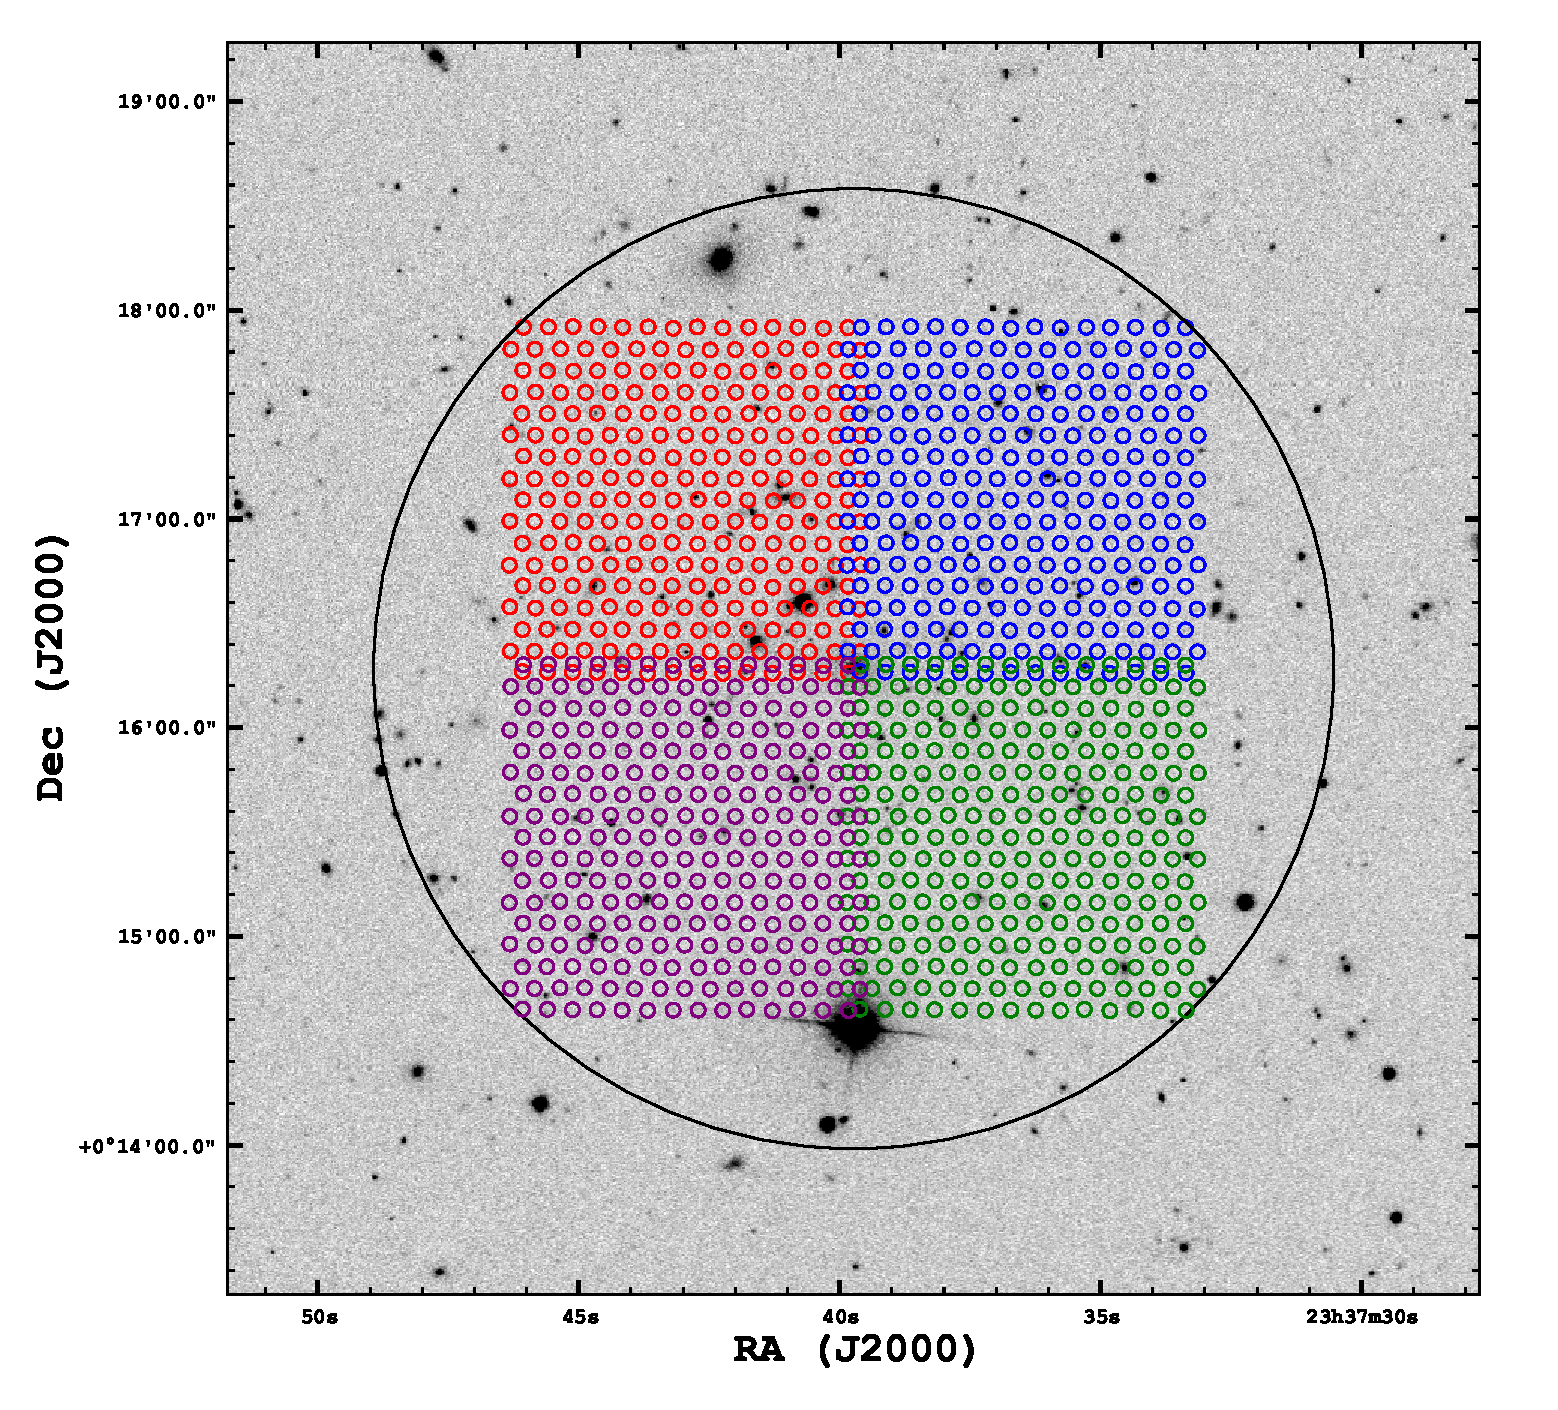
\includegraphics[width=0.6\textwidth]{./figures/pointings.eps} 
			\caption{SDSS r-band image of an optically selected galaxy cluster selected from the SDSS DR8 data. The field is centered on the BCG, which has a measured spectroscopic redshift from SDSS of $z = 0.277$. The large black circle shows the region $R<0.5$ Mpc ($r<2.3'$). Nearly all galaxies within this region are associated with the cluster. The four MS fields (and fiber positions for the first dither position) are overdrawn on the field, illustrating how we survey each cluster.}
			\label{fig:pointings} 
		\end{SCfigure}
		
		\3 We have set exposure times to achieve spectra with signal-to-noise ratios (SNRs) $\sim3$ per spectral element in the continuum for objects with g = 21.3 mag (which corresponds to approximately 0.2L* for cluster galaxies at $z = 0.2$).
\end{outline}

\subsection{Data Reduction}
\begin{outline}[enumerate]
	\1 All data are reduced using \textsc{p3d} \citep{Sandin2010} which is a general IFU reduction pipeline. It uses established techniques to both wavelength calibrate and extract the spectra. We do not flux calibrate our spectra.
	\1 We use wavelength calibration from images of Hg+Cd (for the May, 2012 observations) or Cd+Ne (for all subsequent observations) arc lamps.
	\1 The majority of fibers for any single pointing are empty, we use a $3\sigma$ clipped median selection to identify sky fibers and a simple average to combine them. The result is then subtracted from every fiber. This adequately removes the bulk of sky emission lines, but often fails to completely remove the \ion{O}{1} line at 5577\AA. This line is masked throughout the determination of redshifts. See Figure~\ref{fig:spectrum} for an example of a reduced spectrum.
		\begin{SCfigure} 
			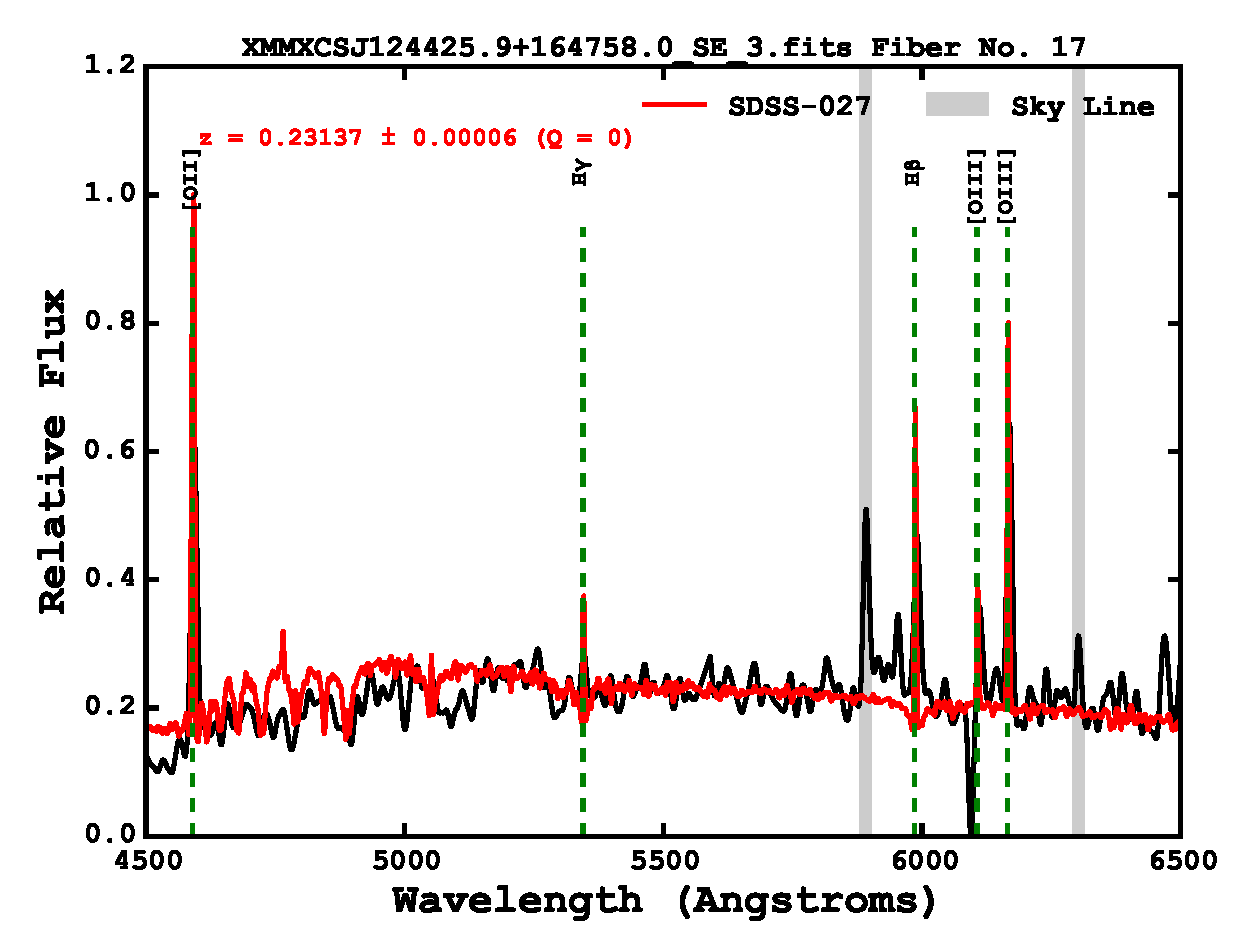
\includegraphics[width=0.6\textwidth]{./figures/spectrum.eps} 
			\caption{Example spectrum of an emission-line cluster galaxy (black line) and template fit (red line) from VIRUS-P on the McDonald 2.7m telescope. The spectrum shows the wavelength range and data quality expected from HETDEX-like spectroscopy, which are sufficient to measure galaxy redshifts.}
			\label{fig:spectrum} 
		\end{SCfigure}
\end{outline}

\subsection{Analysis}
\begin{outline}[enumerate]
	\1 Redshift Catalog
		\2 A redshift solution is determined for each object by cross-correlating \citep{Tonry1979} each of the spectra with galaxy template spectra from the SDSS using the \textsc{xcsao} task in the \textsc{iraf} \textsc{rvsao} package \citep{Kurtz1992}. See Figure~\ref{fig:spectrum} for an example of a fitted spectrum.
	\1 Photometric Catalog
		\2 Each galaxy detection has a corresponding SDSS detection providing photometric information in addition to the measured redshifts. See Figure~\ref{fig:mosaic} for an example of the spectroscopic targets matched to the photometric detections.
		\begin{SCfigure} 
			\includegraphics[width=0.6\textwidth]{./figures/c203p83+41p0_mosaic.eps} 
			\caption{SDSS \sdssr\ image of cluster c203p83+41p0. The symbols show the position of observed galaxies. Blue circles indicate galaxies with $Q=0$ or $Q=1$ spectroscopic redshifts, red squares indicate galaxies where a redshift could not be reliably determined, and the orange diamond corresponds to galaxies with pre-existing redshifts from the SDSS.}
			\label{fig:mosaic} 
		\end{SCfigure}
	\1 Data Quality Control
		\2 For each redshift computed a ``Q'' or quality flag is assigned. $Q=0$ implies high-confidence redshifts, clearly determined by at least two obvious features. See Figure~\ref{fig:spectrum}. Spectra with only a single strong feature (\eg, [\ion{O}{2}] emission) but lie near the correct redshift of the cluster are assigned $Q=1$ and redshifts resulting from enigmatic features are assigned $Q=2$. For the determination of cluster properties we only consider $Q=0$ and $Q=1$ quality flags.
\end{outline}

\subsection{Results}
\begin{outline}[enumerate]
	\1 Cluster Membership
		\2 To reject spurious sources not associated with the any given cluster we employ two methods. For clusters with 20 or more $Q=0$ redshifts we use the  ``shifting gapped" method of \cite{Fadda1996}.
		\2 For galaxy clusters with fewer than 20 $Q=0$ redshifts we employ the method outlined in \cite{Connelly2012,Wilman2005} where we assume an initial velocity dispersion of 500\kms\ and apply both redshift and spatial limits. The number of total redshifts, $Q=0$ redshifts, and confirmed cluster members are given in Table~\ref{tbl:cluster members}.
		\begin{table*}
			\centering
			\caption{Observed clusters with the total number of sources detected, the number of corresponding $Q=0$ redshifts and the number of confirmed cluster members after the confirmation process has been completed. Clusters missing data have technical problems under current investigation.}
			\begin{tabular}{ccccccc}
				\hline
				Cluster & Sources & Q=0 & Members & $z_{c}$ & $\sigma$ (\kms) & $M_{200}$ ($10^{15}$ \Msol) \\
				\hline \hline
		c250p08+46p7 & 62 & 34 & 23 & 0.2256 & 1044\err{196}{131} & 1.75\err{0.6}{0.47} \\
		c203p83+41p0 & 68 & 39 & 26 & 0.2346 & 1364\err{241}{159} & 3.89\err{1.2}{0.96} \\
		c210p2+02p8 & 64 & 33 & 6 & ... & ... & ... \\
		c234p2+24p4 & 38 & 24 & 19 & 0.2265 & 883\err{188}{91} & 1.06\err{0.40}{0.23} \\
		c260p61+32p13 & 61 & 42 & 26 & 0.2256 & 881\err{156}{93} & 1.05\err{0.34}{0.23} \\
		c16p23+0p06& 42 & 24 & 17 & 0.2720 & 1215\err{228}{137} & 2.69\err{0.91}{0.64} \\
		c328p33+0p19 & 28 & 18 & 15 & 0.2165 & 396\err{120}{60} & 0.096\err{5.0}{3.2} \\
		c319p70+0p56 & 47 & 24 & 20 & 0.2760 & 729\err{142}{94} & 0.58\err{2.04}{1.60} \\
		XMMXCSJ124425.9+164758.0 & 24 & 12 & 6 & 0.2349 & 348\err{216}{109} & 0.06\err{5.56}{4.73} \\
		XMMXCSJ125650.2+254803.2 & 15 & 7 & ... & ... & ... & ... \\
		 		\hline
			\end{tabular}
			\label{tbl:cluster members}
		\end{table*}
	\1 Cluster Redshift
		\2 The cluster redshift is the mean redshift of a confirmed member galaxies.
	\1 Line of Sight Velocity Dispersion
		\2 For clusters with at least 15 confirmed members we employ the biweight sample variance \citep{Ruel2014} a modified version of the biweight scale estimator \citep{Beers1990}.
		\2 For galaxy clusters with fewer than 15 members, we employ the gapper estimator \citep{Beers1990} which provides accurate dispersions for groups as small as 5 members \citep{Hou2009}.
	\1 Dynamical Mass
		\2 We use a scaling relation from \cite{Evrard2008,Saro2013, Munari2013} to define the mass enclosed by $r_{200c}$ which has been used in both simulations \citeeg{Old2014}, and observational studies \citeeg{Brodwin2010}.
\end{outline}
\subsection{Calibrating the Observable-Mass Relation}
\begin{outline}[enumerate]
	\1 Richness
		\2 The dominant sources of error on these cosmological parameters from counts of optical clusters are systematic uncertainties on the absolute scale between the cluster mass and optical richness, and the intrinsic scatter in cluster mass at fixed richness.
	\1 X-ray Temperature
		\2 Many (all) of the observed clusters also have X-ray observations. This will allow us a second independent check of the recovered halo masses.
\end{outline}

\section{Timeline to Completion}
\begin{outline}[enumerate]
	\1 Spring 2015
		\2 April
			\3 Work using the Internal Color Dispersion is completed. Published, \cite{Boada2015}.
		\2 May
			\3 HETDEX simulation analysis technical infrastructure is completed. This includes the code to replicate the HETDEX observations and all of the analysis code which calculates the derived quantities, LOSVD, mass, etc. 
			\3 Details outlining the methods used to derive these quantities are added to the paper draft. 
			\3 Details outline the chosen methods are also added to the VIRUS-P paper. 
	\1 Summer 2015
		\2 June
			\3 Details of the direction of thesis work are hammered out.
		\2 July
			\3 Detailed direction of thesis is finalized. 
			\3 Analysis of HETDEX simulations begins in earnest.
			\3 HETDEX paper is written concurrently with analysis.
		\2 August
			\3 Draft of HETDEX paper is completed and sent to co-authors.
			\3 VIRUS-P data is sent through the already existing HETDEX analysis pipeline.
			\3 Writing of the VIURS-P paper begins in earnest.
			\3 Job search preparations begin.
		\2 September
			\3 HETDEX paper is submitted
			\3 VIRUS-P paper is completed and sent to co-authors.
	\1 Fall 2015
		\2 October
			\3 Job applications are in full swing
			\3 VIRUS-P paper is submitted
			\3 Begin dealing with HETDEX referee report
		\2 November
			\3 Job applications?
			\3 VIRUS-P referee report
			\3 Resubmit HETDEX paper
	\1 Winter 2015--2016
		\2 December
			\3 Resubmit VIRUS-P paper
		\2 January
			\3 Apply to Graduate
			\3 Finish any outstanding issues with VIRUS-P paper
			\3 Begin composing thesis
		\2 February
			\3 Write thesis
	\1 Spring 2016
		\2 March
			\3 Defend
		\2 April
			\3 Complete thesis
		\2 May
			\3 Graduate
\end{outline}
\bibliography{master}

\end{document}
